\documentclass[pdflatex,sn-mathphys-num]{sn-jnl}
\usepackage{graphicx}%
\usepackage{amsmath,amssymb,amsfonts}%
\usepackage{amsthm}%
\usepackage{mathrsfs}%
\usepackage{xcolor}%
\usepackage{textcomp}%
\usepackage{booktabs}%
\usepackage{tabularx}%
\usepackage{float}% retained to compile existing table/figure placement markup
\IfFileExists{placeins.sty}{\usepackage{placeins}}{\newcommand{\FloatBarrier}{\clearpage}}%

\floatstyle{ruled}
\newfloat{algorithm}{tbp}{loa}
\floatname{algorithm}{Algorithm}
\makeatletter
\providecommand*{\toclevel@algorithm}{1}
\newcounter{ALG@line}
\newenvironment{algorithmic}[1][0]{%
  \setcounter{ALG@line}{0}%
  \def\ALG@freq{#1}%
  \begin{list}{\ifnum\ALG@freq>0\refstepcounter{ALG@line}\arabic{ALG@line}:\fi}{%
\setlength{\leftmargin}{2.2em}%
\setlength{\labelwidth}{1.8em}%
\setlength{\labelsep}{0.4em}%
\setlength{\itemsep}{2pt}%
\setlength{\parsep}{0pt}%
\setlength{\topsep}{3pt}%
  }%
}{\end{list}}
\newcommand{\Require}{\item[\textbf{Require:}]}
\newcommand{\Ensure}{\item[\textbf{Ensure:}]}
\newcommand{\State}{\item}
\newcommand{\For}[1]{\State \textbf{for} #1 \textbf{do}}
\newcommand{\EndFor}{\State \textbf{end for}}
\makeatother

\theoremstyle{thmstyleone}%
\newtheorem{theorem}{Theorem}[section]
\newtheorem{proposition}[theorem]{Proposition}
\newtheorem{lemma}[theorem]{Lemma}

\theoremstyle{thmstylethree}%
\newtheorem{assumption}[theorem]{Assumption}

\theoremstyle{thmstyletwo}%
\newtheorem{remark}[theorem]{Remark}
\providecommand*{\theHassumption}{\theHtheorem}

\newcommand{\dd}{\mathrm d}
\newcommand{\E}{\mathbb E}
\newcommand{\Q}{\mathbb Q}
\newcommand{\R}{\mathbb R}
\newcommand{\F}{\mathcal F}
\providecommand{\supp}{\operatorname{supp}}
\providecommand{\footnoteA}[1]{\footnote{#1}}
\let\burl\url
\hypersetup{hypertexnames=false}

\makeatletter
\renewenvironment{table}[1][]{%
  \par\addvspace{12pt}%
  \noindent\begin{minipage}{\textwidth}%
  \def\@captype{table}%
  \centering%
  \tablebodyfont%
}{%
  \end{minipage}%
  \par\addvspace{12pt}%
}
\renewenvironment{tablenotes}[1][]{%
  \begin{list}{}{\setlength{\labelsep}{0pt}%
  \setlength{\labelwidth}{0pt}%
  \setlength{\leftmargin}{0pt}%
  \setlength{\rightmargin}{0pt}%
  \setlength{\topsep}{-6pt}%
  \setlength{\itemsep}{2pt}%
  \setlength{\partopsep}{0pt}%
  \setlength{\listparindent}{0em}%
  \setlength{\parsep}{0pt}}%
}{%
  \end{list}%
}
\makeatother

\raggedbottom

\begin{document}

\title[A Hybrid LSMC–PDE Method for Bermudan Option Pricing under the Gatheral Double Mean-Reverting Model]{A Hybrid LSMC–PDE Method for Bermudan Option Pricing under the Gatheral Double Mean-Reverting Model}

\author[1]{\fnm{Mara Kalicanin} \sur{Dimitrov}}\email{mara.kalicanin.dimitrov@mdu.se}
\author*[1]{\fnm{Ying} \sur{Ni}}\email{ying.ni@mdu.se}

\affil*[1]{\orgdiv{Department of Business and Mathematics}, \orgname{M\"{a}lardalen University}, \orgaddress{\postcode{721~23}, \city{V\"{a}ster{\aa}s}, \country{Sweden}}}


\abstract{
We study Bermudan option pricing under the Gatheral Double Mean-Reverting (GDMR) stochastic volatility model. The model features a variance process together with a stochastic long-run mean variance process and allows Constant Elasticity of Variance (CEV)-type exponents in the diffusion coefficients. This model is attractive since it provides a flexible specification for volatility dynamics. However, the pricing of early-exercise derivatives under the GDMR model remains largely unexplored in the literature. To address this challenge, we adapt a Hybrid Least-Squares Monte Carlo–Partial Differential Equation (LSMC–PDE) framework to the GDMR model and provide a detailed model-specific implementation. Conditioning on simulated variance paths, the pricing problem reduces to a one-dimensional problem in the asset price, which is solved by a Fourier-based approach, while the remaining dependence on the variance variables is approximated by least-squares regression. 
%For completeness, we also discuss theoretical properties of the generalized variance dynamics, %including well-posedness and nonnegativity under suitable conditions on the CEV exponents.
Our  numerical experiments demonstrate that the Hybrid LSMC–PDE approach yields accurate pricing estimates and often lower pricing errors than plain LSMC, particularly for low and moderate numbers of simulation paths, showing the benefit of using the model structure in early-exercise option pricing.
}
\keywords{Bermudan option pricing, stochastic volatility, Hybrid LSMC--PDE, least-squares Monte Carlo, Gatheral model}

\maketitle

\section{Introduction}

Bermudan option pricing under stochastic volatility requires repeated
approximation of continuation values defined as conditional expectations of discounted future payoffs. Deterministic Partial Differential Equation (PDE) methods handle this recursion well in low-dimensional Markovian models, but their cost grows quickly when several
volatility factors are present. Under a multi-factor stochastic volatility model, the resulting three or higher dimensional pricing problem becomes increasingly computationally demanding.

Regression-based Monte Carlo approaches for pricing American-style options were developed by Tsitsiklis and Van Roy~\cite{tsitsiklis2001regression} and later popularized through the Least-Squares Monte Carlo (LSMC) method of Longstaff and Schwartz~\cite{longstaff2001valuing}, which is now widely used for pricing options with early exercise features.
Clément, Lamberton, and Protter~\cite{clement2002analysis} analyzed the
convergence of the least-squares regression method for American option pricing.
These methods are flexible, but in stochastic-volatility models the regression approximation of the continuation value function must capture the dependence on both asset and
volatility variables.

Mixed Monte Carlo--PDE methods, which combine simulation with conditional PDE calculations, have shown to be promising for option pricing problems under stochastic-volatility models; see, for example, Loeper and Pironneau~\cite{loeper2009mixed}, Lipp, Loeper, and Pironneau~\cite{lipp2013mixing}, and Cozma and Reisinger~\cite{cozma2017mixed}. More recently, Farahany, Jackson, and Jaimungal~\cite{farahany2020mixing} developed a Hybrid LSMC--PDE method for pricing Bermudan options under stochastic volatility, which forms the methodological basis of the present work. 
Their algorithm simulates the volatility process, solves conditional
asset-direction PDE problems along simulated volatility paths, and then
regresses the resulting conditional values over the volatility state. They also
prove almost-sure convergence for a class of stochastic-volatility models.

We study Bermudan option pricing under the Gatheral-type double mean-reverting stochastic volatility (GDMR) model, introduced in Gatheral~\cite{gatheral2008}, where successful simultaneous calibration to both SPX and VIX option markets was demonstrated. Under this model, the instantaneous variance $v$ mean-reverts to a stochastic variance level $v'$, while $v'$ mean-reverts to a constant long-run level. This double mean-reverting structure is motivated by the
volatility-surface literature (see, e.g., Heston~\cite{heston1993closedform}, Cox, Ingersoll,
and Ross~\cite{cir1985termstructure}, and Gatheral~\cite{gatheral2006volsurface}). 

Despite its appealing modelling properties, the GDMR model does not admit closed-form pricing formulas, even for European options. As a result, calibration in Gatheral~\cite{gatheral2008} was performed using Euler simulation, while Bayer, Gatheral, and Karlsmark~\cite{bayer2013fast} later employed the higher-order Ninomiya--Victoir scheme to improve computational efficiency. Moreover, there has been limited research on Bermudan and American option pricing under this framework. To the best of our knowledge, Haida et al.~\cite{haida2026almost} is among the few studies addressing this problem, proposing a simulation scheme together with a full Least-Squares Monte Carlo (LSMC) method for American option pricing under a double-Heston-type parameterization of the GDMR model. In this work, we aim to fill this gap by developing a Hybrid LSMC--PDE method, adapted from the more general framework of Farahany, Jackson, and Jaimungal~\cite{farahany2020mixing}. This approach is motivated by the computational challenges of applying a full PDE method in the presence of three state variables, while avoiding the need for a full regression approximation of the continuation value as in standard LSMC. Although our discussion focuses on Bermudan option pricing, the framework naturally extends to early-exercise derivatives more broadly through Bermudan approximations of American options.
%% to be added back into a suitable place, it is very strange to appear here. /Ying


We note two advantages of this hybrid method relative to the plain LSMC method.  First, rather than approximating the entire continuation value through a parametric regression approximation, the Hybrid LSMC--PDE method performs regression only partially, leaving the stock-price dependence to be resolved through a conditional pricing PDE. Second, the conditional PDE step naturally produces option values on a grid of stock prices, corresponding to multiple moneyness levels for a fixed strike. This is advantageous for calibration, where option prices across different moneyness values and maturities must be computed repeatedly.

The present paper focuses on adapting the Hybrid LSMC–PDE framework to the GDMR model, motivated by the considerations discussed above. This specialization is nontrivial for the Gatheral double mean-reverting model, because the model has two correlated variance Brownian drivers and Constant Elasticity of Variance (CEV)--type variance coefficients. Our contribution is thus a model-specific formulation and implementation of an existing Hybrid LSMC–PDE framework for the multifactor GDMR setting. First, we derive the Brownian projection and the conditional one-step Gaussian representation needed to apply the existing Hybrid LSMC--PDE framework to the GDMR model. The key model-specific quantities are the correlated Brownian shift $Z_n$, the integrated drift $I_n$, the integrated residual variance $B_n$, and the terminal volatility
state.  

From a computational perspective, we provide a detailed description of the FFT-based numerical implementation and numerical experimental results which may serve as benchmark values for future studies. For the numerical experiments, we use a fixed parameter set based on a calibrated double mean-reverting specification from
Bayer, Gatheral and Karlsmark~\citep{bayer2013fast}. We compare plain LSMC estimator and the Hybrid LSMC--PDE estimator by varying both the Euler step count and the Monte Carlo path budget. Since no closed-form Bermudan option price is available under the GDMR model, the comparisons are made against large-simulation plain LSMC reference prices. Our numerical results indicate that the Hybrid LSMC–PDE method yields accurate pricing estimates and often lower pricing errors than plain LSMC method, particularly for low and moderate numbers of simulation paths.

In addition, we also include a short well-posedness result for the variance subsystem of the GDMR dynamics. This result is not the main contribution of the paper, it is included to make explicit the closed nonnegative variance domain used in the Bermudan recursion and in the conditional construction.








The remainder of the paper is organized as follows. Section~\ref{sec:model}
discusses the GDMR model and gives the
well-posedness result. Section~\ref{sec:conditional_pde} gives the theoretical framework for Bermudan option pricing using the Hybrid LSMC--PDE method and, in particular, derives the
conditional Hybrid LSMC--PDE representation. Section~\ref{sec:hybrid-method} describes
the numerical implementation. Section~\ref{sec:numerical} reports the
experiments. Section~\ref{sec:conclusion} concludes.


\section{Gatheral double mean-reverting model}\label{sec:model}

This section introduces the GDMR model. In this model, the equations for the variance factors do not involve the asset price, while
the asset equation depends on the variance factors. This one-way coupling is
used in Section~\ref{sec:conditional_pde} to obtain the conditional
one-dimensional representation.

\subsection{GDMR dynamics}

Fix a finite horizon $T>0$. Let
$$
(\Omega,\F,(\F_t)_{t\in[0,T]},\Q)
$$
be a filtered probability space satisfying the usual conditions.  Throughout the paper, option pricing is performed under a risk-neutral (equivalent martingale) measure $\Q$ under which the discounted stock price process is assumed to be a true martingale. We assume a deterministic money-market account $B_t=e^{rt}$ where $r$ is the constant risk-free interest rate. Unless otherwise specified, all expectations are taken with respect to the probability measure $\Q$. Furthermore, the notation $\E_\xi[\cdot]$ denotes expectation with respect to the probability distribution of the random variable $\xi$.

The probability space supports a three-dimensional correlated $(\F_t)$-Brownian motion
$$
W=(W^{(1)},W^{(2)},W^{(3)})
$$
with constant quadratic covariations
$$
\langle W^{(i)},W^{(j)}\rangle_t=\rho_{ij}t,\qquad 1\le i,j\le 3.
$$
The matrix $\rho=(\rho_{ij})_{1\le i,j\le 3}$ is symmetric positive
semidefinite and satisfies $\rho_{ii}=1$. We assume $|\rho_{23}|<1$. This ensures that the covariance matrix of the two variance
Brownian drivers, $W^{(2)}$ and $W^{(3)}$, is nonsingular. The assumption is needed in Section~\ref{sec:conditional_pde} where $W^{(1)}$ is decomposed into its projection onto the span of
$(W^{(2)},W^{(3)})$ and an orthogonal residual Brownian component.

We consider the GDMR dynamics of Gatheral~\cite{gatheral2008}, augmented with a risk-free drift term in the stock-price dynamics:
\begin{equation}\label{eq:gdmr}
\begin{aligned}
\dd S_t &= r\,S_t\,\dd t + S_t\sqrt{v_t}\,\dd W^{(1)}_t,\\
\dd v_t &= \kappa_1\,(v'_t - v_t)\,\dd t + \xi_1 v_t^{\delta_1}\,\dd W^{(2)}_t,\\
\dd v'_t &= \kappa_2\,(\theta - v'_t)\,\dd t + \xi_2 (v'_t)^{\delta_2}\,\dd W^{(3)}_t,
\end{aligned}
\end{equation}
where $r\ge0$, $\kappa_1,\kappa_2,\theta,\xi_1,\xi_2>0$, and
$\delta_1,\delta_2\in[1/2,1]$. The factor $v$ is the instantaneous variance and
mean-reverts to the stochastic level $v'$, while $v'$ mean-reverts to the
long-run level $\theta$. The exponents $\delta_1$ and $\delta_2$, referred to as \emph{CEV exponents}, replace the
square-root volatility-of-volatility coefficients by CEV--type powers; the
square-root double mean-reverting model is recovered when
$\delta_1=\delta_2=1/2$.

We further restrict the leverage correlations to satisfy 
$
\rho_{12},
\rho_{13} \in [-1,0].
$
In particular, negative stock-volatility correlations are known to mitigate potential moment explosion effects and support stable martingale behavior in stochastic volatility models as pointed out in Andersen and Piterbarg~\cite{AndersenPiterbarg2007}. This assumption is also consistent with market stylized facts on stock-volatility correlations.


%\begin{assumption}[Pricing martingale]\label{ass:pricing-martingale}
%The discounted stock price $e^{-rt}S_t$ is a true $\Q$-martingale on $[0,T]$.
%\end{assumption}

%This martingale condition is part of the risk-neutral pricing specification.
%The well-posedness result below ensures that the stochastic exponential is well
%defined and that the variance factors remain nonnegative; it does not by itself
%prove the true-martingale property.

\subsection{Well-posedness and nonnegativity}\label{sec:wellposed}



The purpose of this subsection is to state the state-space property of the variance dynamics used later in the pricing construction. Since the variance factors are simulated first and then used in the conditional Hybrid LSMC--PDE step, the factors $v$ and $v'$ must be well defined and nonnegative on the exercise horizon.

The only delicate point is the boundary at zero. When $\delta_i<1$, the CEV coefficients are not Lipschitz at the boundary, so the usual globally Lipschitz SDE argument does not apply directly. This is why we state the well-posedness and nonnegativity result explicitly.

Mishura, Pilipenko, and Ralchenko~\cite{mishura2025gatheral} also study the Gatheral double stochastic-volatility system. In their notation, the variance factors are $X$ and $Y$, corresponding to $v$ and $v'$ in \eqref{eq:gdmr}, with $a_1=b_1=\kappa_1$, $a_2=\kappa_2\theta$, $b_2=\kappa_2$, $\sigma_i=\xi_i$, and $\alpha_i=\delta_i$. They assume strictly positive deterministic initial values and prove strong existence, uniqueness, nonnegativity, and the strong Markov property. Their paper then studies a different issue: whether the volatility factors can remain close to zero, and how a Skorokhod-reflected modification of the internal factor can prevent this behaviour.

We keep the risk-neutral GDMR dynamics in Eq. \eqref{eq:gdmr}, and we use the result only to justify the closed nonnegative variance domain needed for the Bermudan dynamic programming and for the conditional construction in Section~\ref{sec:conditional_pde}. Thus, the theorem is stated in the closed-domain form used in this paper. We do not study the reflected model, near-zero recurrence, strict positivity, or boundary inaccessibility.




%following result to make the closed-state-space property explicit for the GDMR dynamics used in this paper. In particular, we allow $v_0=0$ and $v'_0=0$, although the numerical pricing experiments below use strictly positive initial variance factors.

\begin{assumption}[CEV exponents]\label{ass:delta-range}
Throughout this section we impose
$$
\delta_1,\delta_2\in[1/2,1].
$$
\end{assumption}

Let $x^+=\max\{x,0\}$. For $\delta\in[1/2,1]$, the inequality
$$
\bigl|(x^+)^\delta-(y^+)^\delta\bigr|
\le |x-y|^\delta,\qquad x,y\in\R,
$$
implies that the positive-part diffusion coefficient
$\sigma(x)=\xi(x^+)^\delta$ satisfies
$$
|\sigma(x)-\sigma(y)|
\le \xi |x-y|^\delta,\qquad x,y\in\R.
$$
This is the Yamada-Watanabe modulus condition~\cite{yamada1971uniqueness} in
the one-dimensional form needed below. More explicitly, the condition requires a
nondecreasing function $\varrho$ with $\varrho(0)=0$ and $\varrho(u)>0$ for
$u>0$ such that
$$
|\sigma(x)-\sigma(y)|\le \varrho(|x-y|),\qquad x,y\in\R,
$$
and
$$
\int_0^\varepsilon \frac{\dd u}{\varrho(u)^2}
=
\infty
$$
for sufficiently small $\varepsilon>0$. Here we may take
$\varrho(u)=\xi u^\delta$, since
$$
\int_0^\varepsilon \frac{\dd u}{\varrho(u)^2}
=
\xi^{-2}\int_0^\varepsilon u^{-2\delta}\,\dd u
=
\infty,\qquad \delta\ge\frac12.
$$
The upper bound $\delta\le1$ gives at most linear growth.

The state space used for the GDMR dynamics is
$$
\mathcal D=(0,\infty)\times[0,\infty)^2.
$$

\begin{theorem}[Strong well-posedness and nonnegativity]\label{thm:wellposed}
Assume Assumption~\ref{ass:delta-range}. For every $T>0$ and every initial
state
$$
S_0>0,\qquad v_0\ge0,\qquad v'_0\ge0,
$$
the nonnegative-state system \eqref{eq:gdmr} admits a unique strong solution
$(S_t,v_t,v'_t)_{t\in[0,T]}$ with continuous paths such that
$$
S_t>0,\qquad v_t\ge0,\qquad v'_t\ge0,\qquad
0\le t\le T,\quad \Q\text{-a.s.}
$$
Moreover, for every deterministic initial state in $\mathcal D$, the solution
is a time-homogeneous strong Markov process on $\mathcal D$.
\end{theorem}

Here, the boundary cases $v_0=0$ and $v'_0=0$ are included only to show that the variance system is well defined on the closed nonnegative domain and cannot leave it. They are not used as a modelling choice for calibration or numerical pricing. In the numerical part of the paper, the initial variance factors are strictly positive.

The proof is given in Appendix~\ref{app:proof-wellposed}. It follows the triangular structure of the model.
First, the $v'$-equation is solved, then the $v$-equation is solved with $v'$ as
an adapted input, and finally, the asset equation is recovered from its
stochastic exponential. The same one-way structure is used later in
Subsection~\ref{sec:hybrid-overview} and Proposition~\ref{prop:conditional-gaussian-step}, where the Hybrid LSMC--PDE step conditions on the Brownian increments driving the variance factors.

The lower bound for CEV exponents, $\delta_i\ge1/2$,  is the Yamada-Watanabe threshold for
pathwise uniqueness of power diffusion coefficients. We do not impose a
Feller-type condition, since the theorem proves nonnegativity rather than strict
positivity or boundary inaccessibility.

\section{Bermudan option pricing}\label{sec:conditional_pde}

We now pass from the model dynamics to the one-step continuation calculation in
the Bermudan recursion. The purpose of this section is to explain how the Hybrid LSMC--PDE method is used for the GDMR model and why the Brownian projection is needed.
The Hybrid LSMC--PDE method was developed by Farahany, Jackson, and Jaimungal~\cite{farahany2020mixing} for multidimensional stochastic volatility models. In this paper, our contribution is to adapt that general framework to the GDMR model by deriving the Brownian projection and the resulting one-dimensional conditional log-price representation. We use the
general hybrid-regression convergence theorem in \cite{farahany2020mixing}; the representation derived here provides the
model-specific input needed to apply that theorem.

\subsection{Bermudan stopping problem}\label{sec:bermudan-recursion}

Let
$$
\pi=\{0=t_0<t_1<\cdots<t_M=T\}
$$
be the Bermudan exercise grid. At $t_n$, the payoff is $h_n(S_{t_n})$, where
$h_n:(0,\infty)\to\R$ is Borel. We assume
$$
\E\!\left[
\max_{0\le n\le M}e^{-rt_n}|h_n(S_{t_n})|
\right]<\infty .
$$


We focus on Bermudan put options, with payoff $h_n(s)=(K-s)^+$, for illustrative purposes, since the early exercise feature is generally nontrivial.  Under a nonnegative risk-free interest rate and a non-dividend-paying underlying asset, early exercise of call options is not optimal. Nevertheless, the methodology and discussion below can be readily adapted to Bermudan or American call options in settings where early exercise is possible, such as in the presence of dividends or negative interest rates. 


By Theorem~\ref{thm:wellposed}, the state process
$(S_t,v_t,v'_t)$ is a time-homogeneous Markov process on
$$
\mathcal D=(0,\infty)\times[0,\infty)^2 .
$$
Thus the Bermudan value functions may be defined by backward induction. Write
$$
\Delta t_n:=t_{n+1}-t_n
$$
and set the value function at maturity as
$$
U_M(s,v,w):=h_M(s),
$$
where $w$ denotes the second variance coordinate. For $n=M-1,\ldots,0$, define
$$
\begin{aligned}
C_n(s,v,w)
:=
e^{-r\Delta t_n}
\E\!\left[
U_{n+1}(S_{t_{n+1}},v_{t_{n+1}},v'_{t_{n+1}})
\,\middle|\,
S_{t_n}=s,\ v_{t_n}=v,\ v'_{t_n}=w
\right],
\end{aligned}
$$
and following the dynamic programming principle, the value function at time $t_n$ prior to maturity is
$$
U_n(s,v,w):=\max\{h_n(s),C_n(s,v,w)\}.
$$
The time-zero Bermudan value is
$$
V_0=U_0(S_0,v_0,v'_0).
$$

\subsection{Hybrid decomposition of the continuation value}\label{sec:hybrid-overview}

A plain LSMC method approximates the continuation value in the Bermudan recursion
by regressing simulated discounted next-step values on the current state. In a
stochastic-volatility model this regression is more demanding than in a one-factor
asset model, because the continuation value depends on both the asset level and the
variance state. The Hybrid LSMC--PDE method reduces this regression problem by
using the one-way coupling structure of the dynamics. The variance factors are simulated
first; along each simulated variance path, the remaining conditional expectation in
the asset direction is computed by a one-dimensional PDE step; the resulting
pathwise conditional values are then regressed over the current variance state. The
numerical realization of these steps, including the FFT evaluation and the regression
matrices, is given in Section~\ref{sec:hybrid-method}.

The idea can be written directly at the level of one Bermudan interval. Let $F$ be
a next-step value function; in the backward recursion, $F$ is $U_{n+1}$ or its
numerical approximation. For a current state $(s,v,w)$, define
$$
C_n^F(s,v,w)
=
e^{-r\Delta t_n}
\E\!\left[
F(S_{t_{n+1}},v_{t_{n+1}},v'_{t_{n+1}})
\,\middle|\,
S_{t_n}=s,\ v_{t_n}=v,\ v'_{t_n}=w
\right].
$$
The hybrid method evaluates this conditional expectation in two stages, using
the one-way coupling of the model. The equations for $(v,v')$ do not involve
$S$, so over one exercise interval we may first simulate the Brownian increments
driving the variance factors. Conditioning on these increments fixes the
variance segment and the part of the asset Brownian motion correlated with the
variance drivers. The only remaining asset randomness is the orthogonal
Brownian component. This conditioning is used only inside the one-step
conditional expectation and does not change the information used for the
exercise decision at the exercise dates.

Let $\mathcal H_n$ denote this enlarged conditioning information; its precise
definition is given in the next subsection. The inner, pathwise continuation value is

\begin{equation}\label{eq:innercontval}
    \bar C_n^F(s;\mathcal H_n):= e^{-r\Delta t_n} \E\!\left[ F(S_{t_{n+1}},v_{t_{n+1}},v'_{t_{n+1}})
\,\middle|\, S_{t_n}=s,\mathcal H_n \right].
\end{equation}

For each simulated variance path segment, $\bar C_n^F(\cdot;\mathcal H_n)$ is a
function of the initial asset level. The original continuation value is recovered by the outer conditional expectation
$$
C_n^F(s,v,w) = \E\!\left[ \bar C_n^F(s;\mathcal H_n) \,\middle|\, v_{t_n}=v,\ v'_{t_n}=w
\right].
$$
This expectation is the part approximated by least-squares regression over the current variance state.

To compute the continuation value, we must isolate the part of the asset Brownian motion that remains random after conditioning on $\mathcal H_n$. This is the role of the Brownian projection below. Once this residual component is identified, the conditional asset-price problem becomes one-dimensional in the log-price variable. The conditioning is only an iterated-expectation device and does not change the exercise information at time $t_n$.

\subsection{Brownian projection}

We now make the conditioning information in the preceding decomposition explicit.
Fix an interval $[t_n,t_{n+1}]$ in the Bermudan exercise grid and define
$$
\mathcal H_n := \F_{t_n}
\vee \sigma\!\left( W_s^{(2)}-W_{t_n}^{(2)},
W_s^{(3)}-W_{t_n}^{(3)}: s\in[t_n,t_{n+1}]
\right), 
$$
where $\F_1 \vee \F_2 := \sigma(\F_1 \cup \F_2)$.

Since $v$ and $v'$ are driven only by $W^{(2)}$ and $W^{(3)}$, the path
$(v_s,v'_s)_{s\in[t_n,t_{n+1}]}$ is $\mathcal H_n$-measurable. By assumption $|\rho_{23}|\neq1$, we may project
$W^{(1)}$ onto the span of $(W^{(2)},W^{(3)})$. Set
$$
\Sigma_{23}:=
\begin{bmatrix}
1 & \rho_{23}\\
\rho_{23} & 1
\end{bmatrix},
\qquad
\beta:=\Sigma_{23}^{-1}
\begin{bmatrix}
\rho_{12}\\
\rho_{13}
\end{bmatrix}
=
\begin{bmatrix}
\beta_2\\
\beta_3
\end{bmatrix}.
$$
Equivalently,
\begin{equation}\label{eq:proj-coeffs}
\beta_2=\frac{\rho_{12}-\rho_{13}\rho_{23}}{1-\rho_{23}^2},
\qquad
\beta_3=\frac{\rho_{13}-\rho_{12}\rho_{23}}{1-\rho_{23}^2}.
\end{equation}
The residual variance is
\begin{equation}\label{eq:sigperp}
\begin{aligned}
\sigma_\perp^2
&:=
1-
\begin{bmatrix}\rho_{12}&\rho_{13}\end{bmatrix}
\Sigma_{23}^{-1}
\begin{bmatrix}\rho_{12}\\ \rho_{13}\end{bmatrix} \\
&=
\frac{
1-\rho_{12}^2-\rho_{13}^2-\rho_{23}^2
+2\rho_{12}\rho_{13}\rho_{23}
}{1-\rho_{23}^2}
\ge0 .
\end{aligned}
\end{equation}
When $\sigma_\perp>0$,
$$
B_t^\perp
:=
\frac{W_t^{(1)}-\beta_2W_t^{(2)}-\beta_3W_t^{(3)}}{\sigma_\perp}
$$
is a Brownian motion, and its increments over $[t_n,t_{n+1}]$ are independent
of $\mathcal H_n$. Hence
\begin{equation}\label{eq:orth}
\dd W_t^{(1)}
=\beta_2\,\dd W_t^{(2)}
+\beta_3\,\dd W_t^{(3)}
+\sigma_\perp\,\dd B_t^\perp.
\end{equation}
If $\sigma_\perp=0$, the residual term is absent and the asset Brownian driver
is fully determined by the Brownian drivers of the variance factors.

\subsection{Conditional one-dimensional equation}

Let $X_t:=\log S_t$. Substituting Eq. \eqref{eq:orth} into the asset price equation for $S_t$ in Eq. (\ref{eq:gdmr}) gives
$$
\dd X_t
=\Bigl(r-\tfrac12v_t\Bigr)\dd t
+\sqrt{v_t}\Bigl(\beta_2\,\dd W_t^{(2)}
+\beta_3\,\dd W_t^{(3)}\Bigr)
+\sigma_\perp\sqrt{v_t}\,\dd B_t^\perp .
$$
Define the $\mathcal H_n$-measurable shift
$$
Z_n:=
\int_{t_n}^{t_{n+1}}
\sqrt{v_s}\Bigl(\beta_2\,\dd W_s^{(2)}+
\beta_3\,\dd W_s^{(3)}\Bigr).
$$
For $t\in[t_n,t_{n+1}]$, define also
$$
I_n(t):=\int_t^{t_{n+1}}\Bigl(r-\tfrac12v_s\Bigr)\dd s,
\qquad
B_n(t):=\sigma_\perp^2\int_t^{t_{n+1}}v_s\,\dd s,
$$
and write $I_n:=I_n(t_n)$ and $B_n:=B_n(t_n)$.

\begin{proposition}[Conditional one-step representation]\label{prop:conditional-gaussian-step}
Let $G:\R\times[0,\infty)^2\to\R$ be bounded and Borel. Conditionally on
$\mathcal H_n$, the function
$$
u(t,y)
:=
\E\!\left[
G\!\left(
Y_{t_{n+1}}^{t,y}+Z_n,
v_{t_{n+1}},
v'_{t_{n+1}}
\right)
\,\middle|\,
\mathcal H_n
\right],
$$
where
$$
\dd Y_s^{t,y}
=\Bigl(r-\tfrac12v_s\Bigr)\dd s
+\sigma_\perp\sqrt{v_s}\,\dd B_s^\perp,
\qquad
Y_t^{t,y}=y,
$$
is the bounded mild solution of
$$
\partial_tu+
\Bigl(r-\tfrac12v_t\Bigr)\partial_yu+
\frac12\sigma_\perp^2v_t\partial_{yy}u=0,
\qquad
u(t_{n+1},y)=G(y+Z_n,v_{t_{n+1}},v'_{t_{n+1}}).
$$
Equivalently, for an auxiliary $\xi\sim N(0,1)$,
\begin{equation}\label{eq:gaussian_rep}
u(t,y)
=
\E_\xi\!\left[
G\!\left(
y+Z_n+I_n(t)+\sqrt{B_n(t)}\,\xi,
v_{t_{n+1}},
v'_{t_{n+1}}
\right)
\right],
\end{equation}
with the deterministic interpretation when $B_n(t)=0$.
\end{proposition}

%\noindent\textit{Proof.} 
\begin{proof}
After conditioning on $\mathcal H_n$, the variance
path and the shift $Z_n$ are fixed. If $\sigma_\perp>0$, the only remaining
randomness is the residual Brownian motion; if $\sigma_\perp=0$, the
conditional step is deterministic. The conditional
Feynman-Kac formula gives the backward Kolmogorov equation. Since the
coefficients are independent of $y$, the terminal log-price is Gaussian with
mean $y+I_n(t)$ and variance $B_n(t)$, which gives the displayed formula.
\end{proof}
For an asset-space next-step value function $F$ and
$G(y,v,w):=F(e^y,v,w)$, the pathwise quantity defined by Eq. \eqref{eq:innercontval} in
Subsection~\ref{sec:hybrid-overview} is
$$
\bar C_n^F(s;\mathcal H_n)=e^{-r\Delta t_n}u(t_n,\log s).
$$
Thus the conditional asset step depends on the sampled
$(W^{(2)},W^{(3)})$-path over $[t_n,t_{n+1}]$ only through
$$
Z_n,\qquad I_n,\qquad B_n,\qquad v_{t_{n+1}},\qquad v'_{t_{n+1}},
$$
while $(v_{t_n},v'_{t_n})$ is the state used in the outer regression.

\subsection{Connection with the hybrid convergence theorem}\label{sec:as_convergence}

The almost-sure convergence theorem for the Hybrid LSMC--PDE regression is proved in Farahany, Jackson, and Jaimungal~\cite{farahany2020mixing}. The preceding subsections identify the model-specific ingredients needed to apply that theorem.

First, the asset equation is multiplicative. For $0\le t<u\le T$,
$$
S_u=S_tR_{t,u},
$$
where
$$
R_{t,u}
=
\exp\left(
\int_t^u\left(r-\frac12v_s\right)\,\dd s
+
\int_t^u\sqrt{v_s}\,\dd W_s^{(1)}
\right).
$$
Thus the return factor $R_{t,u}$ depends on the Brownian and variance paths,
but not on the value of $S_t$.

Second, Proposition~\ref{prop:conditional-gaussian-step} shows that, on each
Bermudan interval, the sampled $(W^{(2)},W^{(3)})$-path enters the conditional
asset-price step only through the finite-dimensional statistic
$$
\Theta_n
:=
(V_n,V_{n+1},Z_n,I_n,B_n),
\qquad
V_n=(v_{t_n},v'_{t_n}).
$$
Because the variance equations do not involve $S$, the model is one-way
coupled. Hence we can apply the hybrid convergence theorem of
\cite[Theorem~1]{farahany2020mixing}.

The remaining assumptions in the cited convergence theorem are stabilizing assumptions on the least-squares regression. In the numerical implementation below, these are enforced by working on the compact volatility rectangle $\mathcal D_v$ in Eq. \eqref{eq:vol-domain}, using a bounded volatility basis on that rectangle as in Eq. \eqref{eq:vol-basis}, and replacing the sample Gram inverse by the bounded inverse $[A_n^N]^{-1}_R$ in Eq. \eqref{eq:estimated_coeff}. The finite log-price grid $\mathcal S_h$ provides the corresponding compact asset domain
for the conditional PDE step. Thus, the convergence theorem is applied to the same stabilized regression used in Section~\ref{sec:hybrid-method}, rather than to a separate truncated algorithm.

Under these stabilized choices, and assuming the population Gram matrices are
nonsingular, the hybrid regression coefficients converge almost surely by
\cite[Theorem~1]{farahany2020mixing}. Consequently, for each fixed asset level,
the fitted continuation values converge uniformly on the chosen compact
volatility domain.
\section{Numerical implementation}
\label{sec:hybrid-method}

The numerical experiments use the following implementation. The conditional
representation is derived in Section~\ref{sec:conditional_pde}; here we specify the grids, variance discretization, accumulated path statistics, FFT step, regression step, and time-zero estimator. We use this implementation because the conditional PDE admits a Gaussian structure in its solution, allowing the shift operation in the conditional formulation to be handled efficiently in Fourier space. In addition, the FFT implementation appears computationally advantageous in our numerical experiments.


%These numerical choices are separate from the convergence statement quoted in Section~\ref{sec:conditional_pde}.



\subsection{Grids and basis functions}
Let
$$
\pi=\{0=t_0<t_1<\cdots<t_M=T\}
$$
be the Bermudan exercise grid, and let $h_n$ denote the exercise payoff at
$t_n$. We work on a uniform log-price grid
$$
y_i=y_{\min}+(i-1)\Delta y,
\qquad
\Delta y=\frac{y_{\max}-y_{\min}}{N_S-1},
\qquad
i=1,\ldots,N_S,
$$
and set
$$
s_i=e^{y_i},
\qquad
\mathcal S_h:=\{s_1,\ldots,s_{N_S}\}.
$$
The interval $[y_{\min},y_{\max}]$ is chosen large enough to contain the
relevant asset values used in the computation.

For the volatility variables, write $w=v'$. We work on the compact volatility rectangle
\begin{equation}\label{eq:vol-domain}
\mathcal D_v=[0,v_{\max}]\times[0,w_{\max}]\subset[0,\infty)^2 .
\end{equation}
The regression basis is chosen as a vector of continuous functions that are bounded on this rectangle,
\begin{equation}\label{eq:vol-basis}
\phi=(\phi_1,\ldots,\phi_{d_B}), \qquad \sup_{(v,w)\in\mathcal D_v}|\phi_k(v,w)|<\infty,
\qquad k=1,\ldots,d_B.
\end{equation}
For the convergence statement, the numerical basis may be viewed as the restriction to $\mathcal D_v$ of compactly supported continuous functions on the full volatility state space; this extension does not affect the computed regression, since the regression is evaluated only on $\mathcal D_v$.

Once chosen, the domain $\mathcal D_v$ and the basis functions are fixed before
the training regression.

At each exercise date, we approximate the continuation value by a separable
regression form
$$
c_n(s,v,w)\approx a_n(s)\cdot\phi(v,w),
\qquad
a_n(s)\in\R^{d_B}.
$$
Numerically, the coefficient vectors $a_n(s)$ are computed only at the grid points
$s_i\in\mathcal S_h$. Off-grid asset values are evaluated by interpolation in the
log-price coordinate.

\subsection{Variance simulation and path statistics}
Let
$$
0=\tau_0<\tau_1<\cdots<\tau_L=T
$$
be an Euler simulation grid containing all exercise dates in the Bermudan exercise grid $\pi$. Write
$$
\Delta\tau_\ell:=\tau_{\ell+1}-\tau_\ell.
$$
For each path $j$, simulate correlated Gaussian increments
$$
(\Delta W_{\ell}^{(2),j},\Delta W_{\ell}^{(3),j})
$$
with variances $\Delta\tau_\ell$ and covariance
$\rho_{23}\Delta\tau_\ell$. To simulate the variance processes, we adopt a standard positivity-preserving truncated Euler scheme of the form:
$$
\begin{aligned}
\bar w_\ell^j&:=(w_\ell^j)^+,
\qquad
\bar v_\ell^j:=(v_\ell^j)^+,\\
w_{\ell+1}^j
&:=
\left[
w_\ell^j+\kappa_2(\theta-\bar w_\ell^j)\Delta\tau_\ell
+\xi_2(\bar w_\ell^j)^{\delta_2}\Delta W_{\ell}^{(3),j}
\right]^+,\\
v_{\ell+1}^j
&:=
\left[
v_\ell^j+\kappa_1(\bar w_\ell^j-\bar v_\ell^j)\Delta\tau_\ell
+\xi_1(\bar v_\ell^j)^{\delta_1}\Delta W_{\ell}^{(2),j}
\right]^+.
\end{aligned}
$$
For each exercise interval $[t_n,t_{n+1}]$, the path statistics are accumulated
over the Euler substeps contained in that interval:
$$
\begin{aligned}
Z_n^j
&:=
\sum_{\tau_\ell\in[t_n,t_{n+1})}
\sqrt{\bar v_\ell^j}
\left(
\beta_2\Delta W_{\ell}^{(2),j}
+
\beta_3\Delta W_{\ell}^{(3),j}
\right),\\
I_n^j
&:=
\sum_{\tau_\ell\in[t_n,t_{n+1})}
\left(r-\frac12\bar v_\ell^j\right)\Delta\tau_\ell,\\
B_n^j
&:=
\sigma_\perp^2
\sum_{\tau_\ell\in[t_n,t_{n+1})}
\bar v_\ell^j\Delta\tau_\ell .
\end{aligned}
$$
Here the projection coefficients $\beta_2,\beta_3$ and the residual volatility coefficient $\sigma_\perp$ are given by Eqs.~\eqref{eq:proj-coeffs} and~\eqref{eq:sigperp}, respectively. The left-point rule is natural for $Z_n^j$, since $Z_n^j$ approximates a stochastic integral evaluated with left endpoints. The same left-point values are used for $I_n^j$ and $B_n^j$ for consistency with the Euler  simulation, and the same increments $\Delta W_{\ell}^{(2),j},\Delta W_{\ell}^{(3),j}$ are used in the variance updates and in $Z_n^j$.

\subsection{Pathwise FFT propagation and regression}
Fix $n\in\{0,\ldots,M-1\}$. Here $\widehat V_{n+1}^N$ denotes the numerical
Bermudan value surface already available from the next exercise date in the
backward recursion. At maturity this surface is initialized by the payoff function
$$
\widehat V_M^N(s_i,v,w)=h_M(s_i).
$$
At earlier exercise dates it is the previously updated surface
$$
\begin{aligned}
\widehat V_{n+1}^N(s_i,v,w)
&=
\max\{h_{n+1}(s_i),\widehat C_{n+1}^N(s_i,v,w)\},\\
\widehat C_{n+1}^N(s_i,v,w)
&=
a_{n+1}^N(s_i)\cdot\phi(v,w).
\end{aligned}
$$
Thus $\widehat V_{n+1}^N$ is already available before the following pathwise
propagation step. For each Monte Carlo path $j$, the simulated Brownian
increments driving the variance factors on $[t_n,t_{n+1}]$ determine the
endpoint state
$$
(v_{t_{n+1}}^j,w_{t_{n+1}}^j)
$$
and the statistics $Z_n^j,I_n^j,B_n^j$. Define the terminal grid function
$$
g_{n+1}^j(y_i)
:=
\widehat V_{n+1}^N
\left(e^{y_i},v_{t_{n+1}}^j,w_{t_{n+1}}^j\right),
\qquad i=1,\ldots,N_S.
$$
By the Gaussian representation Eq. (\ref{eq:gaussian_rep}) in Section~\ref{sec:conditional_pde},
$$
u_n^j(y)
=
\E_\xi\!\left[
g_{n+1}^j
\left(
y+Z_n^j+I_n^j+\sqrt{B_n^j}\xi
\right)
\right],
\qquad \xi\sim N(0,1).
$$
With the Fourier convention
$$
\mathcal F f(\omega)
=
\int_{\R}e^{-\mathrm i\omega y}f(y)\,\dd y,
$$
we obtain
$$
\mathcal F u_n^j(\omega)
=
\mathcal F g_{n+1}^j(\omega)
\exp\left(
\mathrm i\omega Z_n^j+\mathrm i\omega I_n^j-\frac12\omega^2B_n^j
\right).
$$
Define
$$
\Psi_n^j(\omega)
:=
\mathrm i\omega Z_n^j+\mathrm i\omega I_n^j-\frac12\omega^2B_n^j.
$$
On the uniform log-price grid, the FFT implementation is
\begin{equation}
u_n^j(\cdot)
\approx
\operatorname{FFT}^{-1}
\left(
\operatorname{FFT}[g_{n+1}^j]\,
\exp(\Psi_n^j)
\right),
\label{eq:fft-recursion}
\end{equation}
where the exponential is applied pointwise at the discrete Fourier frequencies.
The FFT input is the unshifted terminal grid $g_{n+1}^j$; the correlated shift
$Z_n^j$ is included only through the multiplier. Equivalently, one may shift the
terminal grid first and omit $\mathrm i\omega Z_n^j$, but the two conventions
must not be combined. If $B_n^j=0$, the conditional propagation reduces to the
deterministic log-price shift $Z_n^j+I_n^j$.

The pathwise pre-surface on the asset grid is
$$
\widehat C_n^j(s_i)
:=
e^{-r\Delta t_n}u_n^j(y_i),
\qquad i=1,\ldots,N_S.
$$

The regression step is performed at each exercise date $t_n$,
$n=M-1,\ldots,1$, and at each asset grid point $s_i$. It estimates the
dependence of the pathwise pre-surface $\widehat C_n^j(s_i)$ on the current
volatility state. Define
$$
V_n^j:=(v_{t_n}^j,w_{t_n}^j).
$$
The sample Gram matrix is
$$
A_n^N
:=
\frac1N\sum_{j=1}^N
\phi(V_n^j)\phi(V_n^j)^\top,
$$
and the right-hand side for the grid point $s_i$ is
$$
b_n^N(s_i)
:=
\frac1N\sum_{j=1}^N
\phi(V_n^j)\widehat C_n^j(s_i).
$$
For numerical stability, we use the truncated inverse
\begin{equation}\label{eq:estimated_coeff}
[A]^{-1}_R
:=
\begin{cases}
A^{-1}, & \text{if $A$ is invertible and }\|A^{-1}\|\le R,\\
0,  & \text{otherwise.}
\end{cases}
\end{equation}
Then set
\begin{equation}
a_n^N(s_i):=[A_n^N]^{-1}_R b_n^N(s_i).
\label{eq:lsq}
\end{equation}
The fitted continuation surface is
$$
\widehat C_n^N(s_i,v,w)
:=
a_n^N(s_i)\cdot\phi(v,w),
$$
and the updated price for the Bermudan option is
$$
\widehat V_n^N(s_i,v,w)
:=
\max\left\{
h_n(s_i),
\widehat C_n^N(s_i,v,w)
\right\}.
$$
Starting from
$$
\widehat V_M^N(s_i,v,w):=h_M(s_i),
$$
the recursion is performed backward for $n=M-1,\ldots,1$. The fitted functions
are defined at the asset grid points and extended to off-grid asset values by
log-price interpolation.

\subsection{Time-zero estimator and pseudocode}
At $t_0=0$, the initial volatility state is fixed, so no regression is needed. After $\widehat V_1^N$ has been fitted, the time-zero
continuation value is evaluated on the asset grid by averaging first-step
pathwise pre-surfaces:
$$
\widehat C_0^N(s_i)
:=
\frac1N
\sum_{j=1}^{N}
\widehat C_0^j(s_i).
$$
The averaged grid values define $\widehat C_0^N$ on the asset grid; off-grid
values are evaluated by the log-price interpolation convention stated above.
Thus $\widehat C_0^N(S_0)$ denotes the averaged continuation value at the
initial asset price, and the Hybrid LSMC--PDE estimator is
\begin{equation}\label{eq:hybrid_est}
\widehat V_0^N(S_0)
=
\max\left\{
h_0(S_0),
\widehat C_0^N(S_0)
\right\}.
\end{equation}
Note that the present implementation has the advantage that option prices are computed simultaneously for multiple initial stock prices on the stock-price grid, equivalently for multiple moneyness levels since the strike price $K$ is fixed, which is particularly desirable for calibration. In contrast, a plain LSMC approach typically produces the option price corresponding to a single initial stock price in each run.

The implementation of the Hybrid LSMC--PDE method is summarized in Algorithm~\ref{alg:hybrid-LSMC--PDE}.
\begin{algorithm}[H]
\caption{Hybrid LSMC--PDE recursion}\label{alg:hybrid-LSMC--PDE}
\begin{algorithmic}[1]
\Require Exercise grid $\{t_n\}_{n=0}^M$, Euler grid containing the exercise dates, log-price grid $\{y_i\}_{i=1}^{N_S}$, volatility domain $\mathcal D_v$, basis $\phi$, truncation level $R$, and path count $N$
\Ensure Hybrid LSMC--PDE estimator $\widehat V_0^N(S_0)$ and fitted continuation surfaces $\widehat C_n^N$
\State Simulate $N$ training paths of the variance factors on the Euler grid.
\State Store exercise-date volatility states and accumulate $Z_n^j$, $I_n^j$, and $B_n^j$ over each interval $[t_n,t_{n+1}]$.
\State Set $\widehat V_M^N(s_i,v,w)\gets h_M(s_i)$ on $\mathcal S_h\times\mathcal D_v$.
\For{$n=M-1,\ldots,1$}
\For{$j=1,\ldots,N$}
\State Compute $\{\widehat C_n^j(s_i)\}_{i=1}^{N_S}$ using the unshifted terminal grid $g_{n+1}^j$ in Eq. \eqref{eq:fft-recursion}, with $Z_n^j$ included only through the multiplier $\exp(\Psi_n^j)$; do not pre-shift $g_{n+1}^j$ by $Z_n^j$.
\EndFor
\For{each $s_i\in\mathcal S_h$}
\State Compute $b_n^N(s_i)$ and $a_n^N(s_i)$ by the truncated-inverse regression Eq. \eqref{eq:lsq}.
\EndFor
\State Set $\widehat C_n^N(s_i,v,w)\gets a_n^N(s_i)\cdot\phi(v,w)$ for all $s_i\in\mathcal S_h$.
\State Set $\widehat V_n^N(s_i,v,w)\gets\max\{h_n(s_i),\widehat C_n^N(s_i,v,w)\}$ for all $s_i\in\mathcal S_h$.
\EndFor
\State Compute the first-step pre-surfaces $\widehat C_0^j(s_i)$ for $j=1,\ldots,N$ using the simulated paths on $[t_0,t_1]$.
\State Set $\widehat C_0^N(s_i)\gets N^{-1}\sum_{j=1}^{N}\widehat C_0^j(s_i)$.
\State Evaluate $\widehat C_0^N(S_0)$ from the averaged continuation grid at $y=\log S_0$, using linear interpolation if needed.
\State \textbf{return} $\widehat V_0^N(S_0)=\max\{h_0(S_0),\widehat C_0^N(S_0)\}$.
\end{algorithmic}
\end{algorithm}
\section{Numerical experiments}\label{sec:numerical}


For numerical illustration, we consider Bermudan put pricing experiments using the fixed parameter set in Table~\ref{tab:parameter-setup}.  Since no closed-form solution is available for Bermudan option prices under the GDMR model, we compare the plain LSMC method~\cite{longstaff2001valuing} and the Hybrid LSMC--PDE estimator in Eq.~\eqref{eq:hybrid_est} against large-simulation LSMC reference prices using relative errors computed with respect to these reference prices. Although the reference prices are not exact solutions, they serve as numerical benchmarks throughout the paper. For simplicity, we refer to these benchmark-relative deviations as relative errors.

%and used to construct the error bars in the figures.

\subsection{Experimental setting and reference values}

Table~\ref{tab:parameter-setup} reports the fixed GDMR parameter set and
numerical settings used in the experiments.
\begin{table}[htbp]
\centering
\caption{Parameter set and numerical settings used in the pricing experiments.}
\label{tab:parameter-setup}
\begin{threeparttable}
\small
\begin{tabularx}{0.94\textwidth}{@{}l c X@{}}
\toprule
Symbol & Value & Interpretation \\
\midrule
$S_0$ & 100 & initial asset price \\
$v_0$ & 0.114 & initial instantaneous variance factor \\
$v'_0$ & 0.110 & initial secondary variance factor \\
$r$ & 0.02 & risk-free rate \\
$T$ & 1.0 & maturity in years \\
$\kappa_1$ & 5.5 & mean-reversion speed of $v_t$ toward $v'_t$ \\
$\kappa_2$ & 0.1 & mean-reversion speed of $v'_t$ toward $\theta$ \\
$\theta$ & 0.078 & long-run variance level \\
$\xi_1$ & 2.689 & volatility scale of the first variance factor \\
$\xi_2$ & 0.502 & volatility scale of the second variance factor \\
$\delta_1$ & 0.94 & CEV exponent of the first variance factor \\
$\delta_2$ & 0.94 & CEV exponent of the second variance factor \\
$\rho_{12}$ & -0.982 & correlation between the first and second Brownian drivers \\
$\rho_{13}$ & -0.727 & correlation between the first and third Brownian drivers \\
$\rho_{23}$ & 0.590 & correlation between the second and third Brownian drivers \\
\addlinespace
\multicolumn{3}{@{}l}{\textit{Fixed numerical setting}} \\
$N_{\mathrm{ex}}$ & 12 &  exercise dates after $t_0$, including maturity \\
$K$ & $\{70,80,90,100,110\}$ & strike prices used in all experiments \\
$N_S$ & 301 & asset-grid points in the conditional PDE solver \\
$(y_{\min},y_{\max})$ & $(\log (0.30S_0),\log(3.5\max \left(S_0, K\right)))$ & lower and upper log-price grid bounds \\
%$(M_{\mathrm{ref}},N_{\mathrm{ref}})$ & $(1200,1{,}200{,}000)$ & reference LSMC step count and path budget \\
\botrule
\end{tabularx}
\end{threeparttable}
\end{table}

%The LSMC reference prices are reported in Table~\ref{tab:reference-prices}. 
A volatility truncation quantile $q_v=0.999$ is used to choose the bounds
$v_{\max}$ and $w_{\max}$ in the compact volatility domain
$\mathcal D_v$ in Eq.~\eqref{eq:vol-domain}. Thus, $v_{\max}$ and $w_{\max}$ are chosen so that approximately $99.9\%$ of
the simulated values of $v$ and $v'$ at the exercise dates lie below the
corresponding bounds, truncating only the upper $0.1\%$ tail. The Hybrid
LSMC--PDE grid and truncation settings are kept fixed throughout all
experiments.

The mean-reversion, volatility-scale, initial-variance, and correlation
parameters are taken from the calibrated double mean-reverting specification of
Bayer, Gatheral and Karlsmark~\citep{bayer2013fast}. Their calibration assumes
$r=0$. In the present Bermudan pricing experiments we keep those variance and
correlation parameters, set $r=0.02$, and use
$\delta_1=\delta_2=0.94$ for the CEV--type generalization. Thus the numerical
section is not a new calibration study; it uses a parameter set from the double
mean-reverting volatility literature as a fixed test case.
The correlation assumptions used in Section~\ref{sec:conditional_pde} are
satisfied. In particular, $|\rho_{23}|<1$ and $\rho_{1,2}, \rho_{1,3} \in [-1,0]$.

The plain LSMC regressions use a cubic $16$-term basis
$$
1,x,y,z,x^2,y^2,z^2,xy,xz,yz,x^3,y^3,z^3,p,p^2,p^3,
$$
where $x=S/S_0$, $y=v/\theta$, $z=v'/\theta$, and
$p=(K-S)^+/K$. The hybrid regressions use a volatility-only cubic basis
$$
1,\tilde{y},\tilde{z},\tilde{y}^2,\tilde{y}\tilde{z},\tilde{z}^2,\tilde{y}^3,\tilde{y}^2\tilde{z},\tilde{y}\tilde{z}^2,\tilde{z}^3,
$$
where
$
\tilde{y}=\min(v,v_{\max})/v_{\max} \text{ and }
\tilde{z}=\min(v',v'_{\max})/v'_{\max}.$

%The smooth compact-support assumption in %Subsection~\ref{sec:as_convergence} is part of the convergence %statement.

The reference prices, denoted by $V^{\mathrm{ref}}$ and reported in Table~\ref{tab:reference-prices}, are large-simulation plain LSMC estimates computed using $1200$ Euler steps and $1{,}200{,}000$ simulation paths. The table also reports empirical Monte Carlo standard errors and associated 95\% confidence intervals. In subsequent relative-error calculations and plots, only $V^{\mathrm{ref}}$ is used as the benchmark, while the associated standard errors and confidence intervals are included for information only.

For an estimator $V$ and reference price $V^{\mathrm{ref}}$, we report the relative error
$$
\varepsilon_{\mathrm{rel}}
:=
\left| \frac{V-V^{\mathrm{ref}}}{V^{\mathrm{ref}}} \right|,
$$
where $V^{\mathrm{ref}}$ is treated as fixed. To visualize the statistical variability of the estimators in the relative-error space, error bars in the relative-error plots are obtained by mapping the 95\% confidence intervals $[V_{\mathrm{left}},V_{\mathrm{right}}]$ of the estimators through
\[
V \mapsto \left| \frac{V - V^{\mathrm{ref}}}{V^{\mathrm{ref}}}\right|.
\]



\begin{table}[htbp]
\centering
\caption{LSMC reference values for the parameter set in Table~\ref{tab:parameter-setup}.}
\label{tab:reference-prices}
\small
\begin{tabularx}{0.82\textwidth}{@{}cccc@{}}
\toprule
$K$ & Reference price ($V^{\mathrm{ref}}$) & Std. error & 95\% confidence interval \\
\midrule
70 & 2.522851 & 0.007103 & [2.508929, 2.536773] \\
80 & 4.298933 & 0.009345 & [4.280617, 4.317249] \\
90 & 6.942119 & 0.011774 & [6.919042, 6.965196] \\
100 & 10.682037 & 0.014105 & [10.654391, 10.709683] \\
110 & 15.743520 & 0.015757 & [15.712636, 15.774404] \\
\botrule
\end{tabularx}
\end{table}

\subsection{Fixed path budget and varying Euler steps}

The first experiment keeps the Monte Carlo path budget fixed and varies the number of
Euler time steps. The two path budgets are $20{,}000$ and $60{,}000$, and
both methods are evaluated at $24,48,72,$ and $96$ Euler steps. This
experiment tests the sensitivity of the estimators to the Euler
discretization.

For $20{,}000$ paths, the relative errors of the plain LSMC estimator over the full step-sweep grid range from $0.344\%$ to $8.645\%$, while those of the Hybrid LSMC--PDE estimator range from 
$0.019\%$ to $7.459\%$. Figure~\ref{fig:step-sweep-20k} reports the strike-wise
relative errors. 

%The corresponding price grids are reported in Appendix~\ref{app:price-grids}.

\begin{figure}[H]
\centering
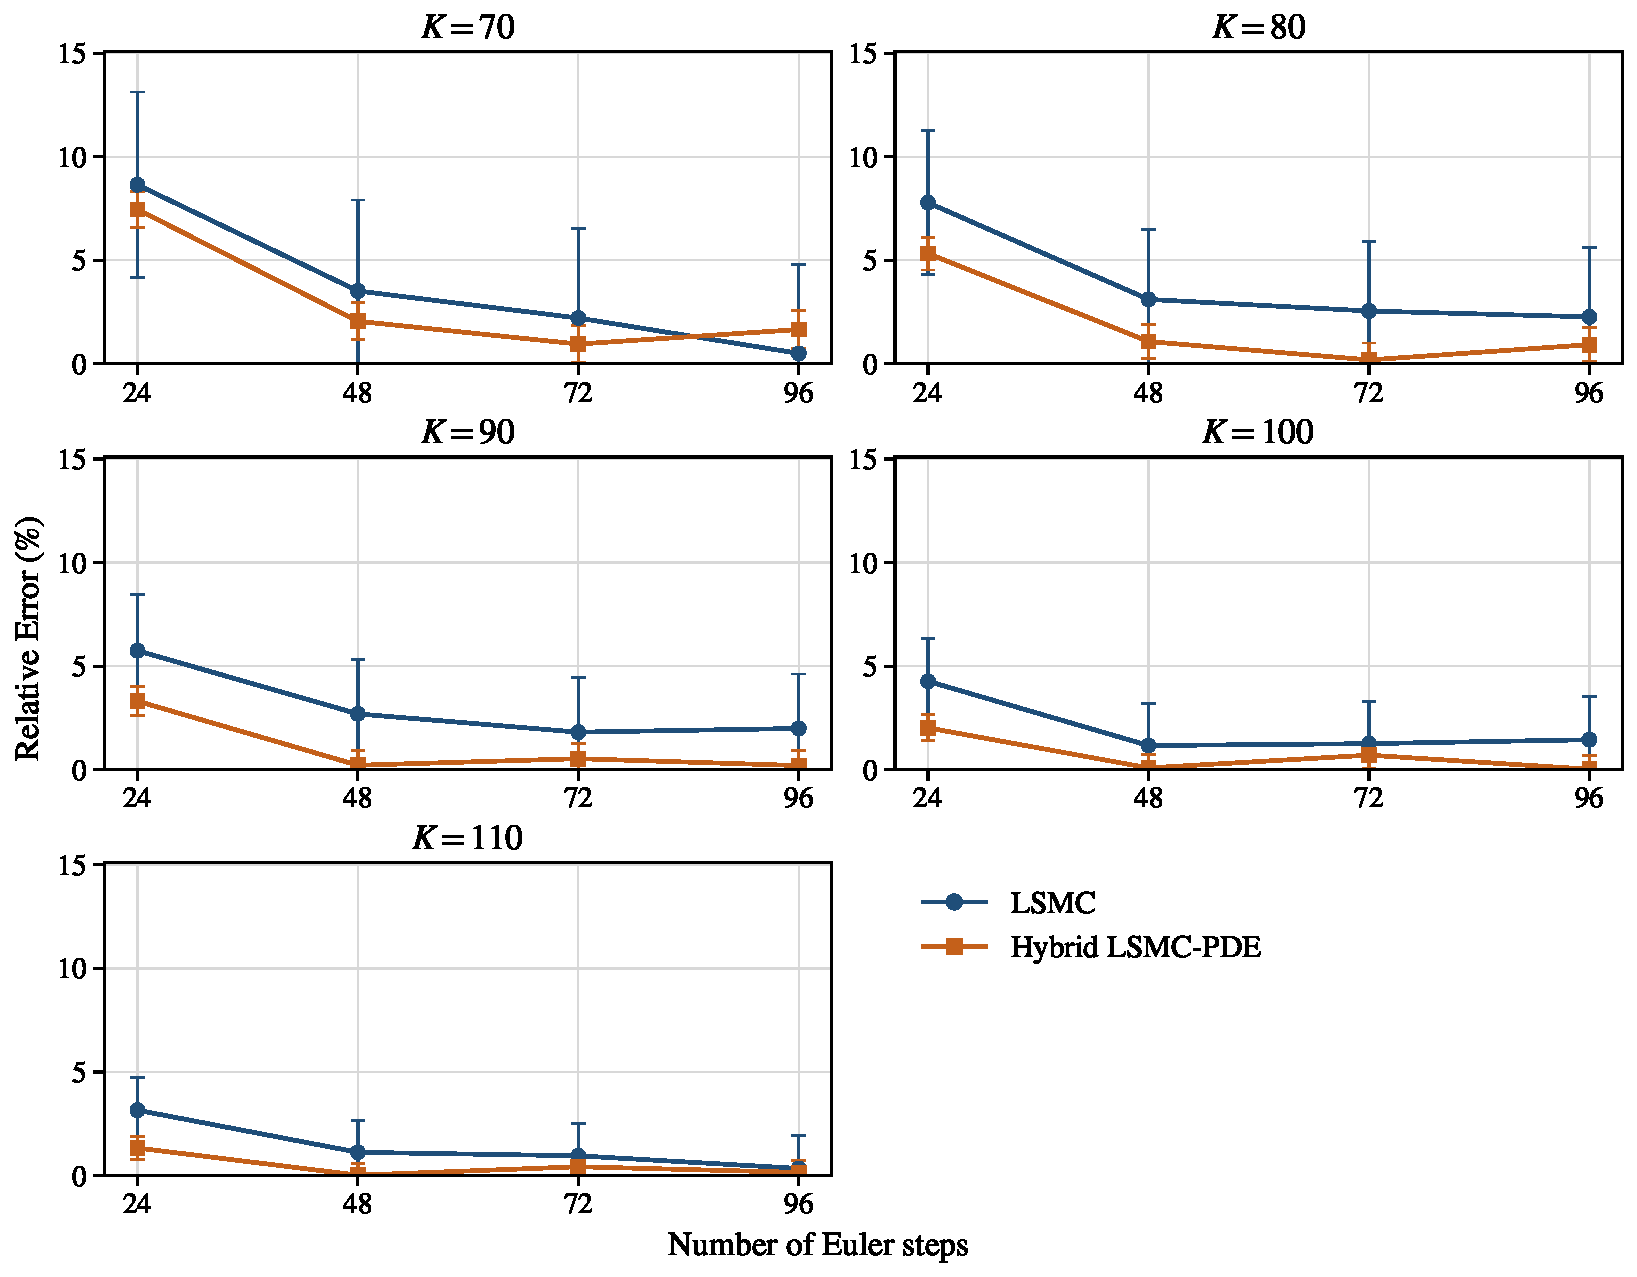
\includegraphics[width=\textwidth]{../Figures/step_sweep_20k_direct_relative_error.pdf}
\caption{Relative errors with associated error bars for  $20{,}000$-path step-sweep experiment.}
\label{fig:step-sweep-20k}
\end{figure}

For $60{,}000$ paths, the same design gives relative errors of the plain LSMC estimator ranging from $0.102\%$ to $7.720\%$, while those of the Hybrid LSMC--PDE estimator range from $0.028\%$ to $7.857\%$. Figure~\ref{fig:step-sweep-60k} reports the corresponding strike-wise relative errors. The Hybrid LSMC--PDE estimator does not give a
smaller relative error in every step-count configuration, but it gives smaller
relative errors in most of the reported configurations, with the clearest
differences at the intermediate step levels.

\begin{figure}[H]
\centering
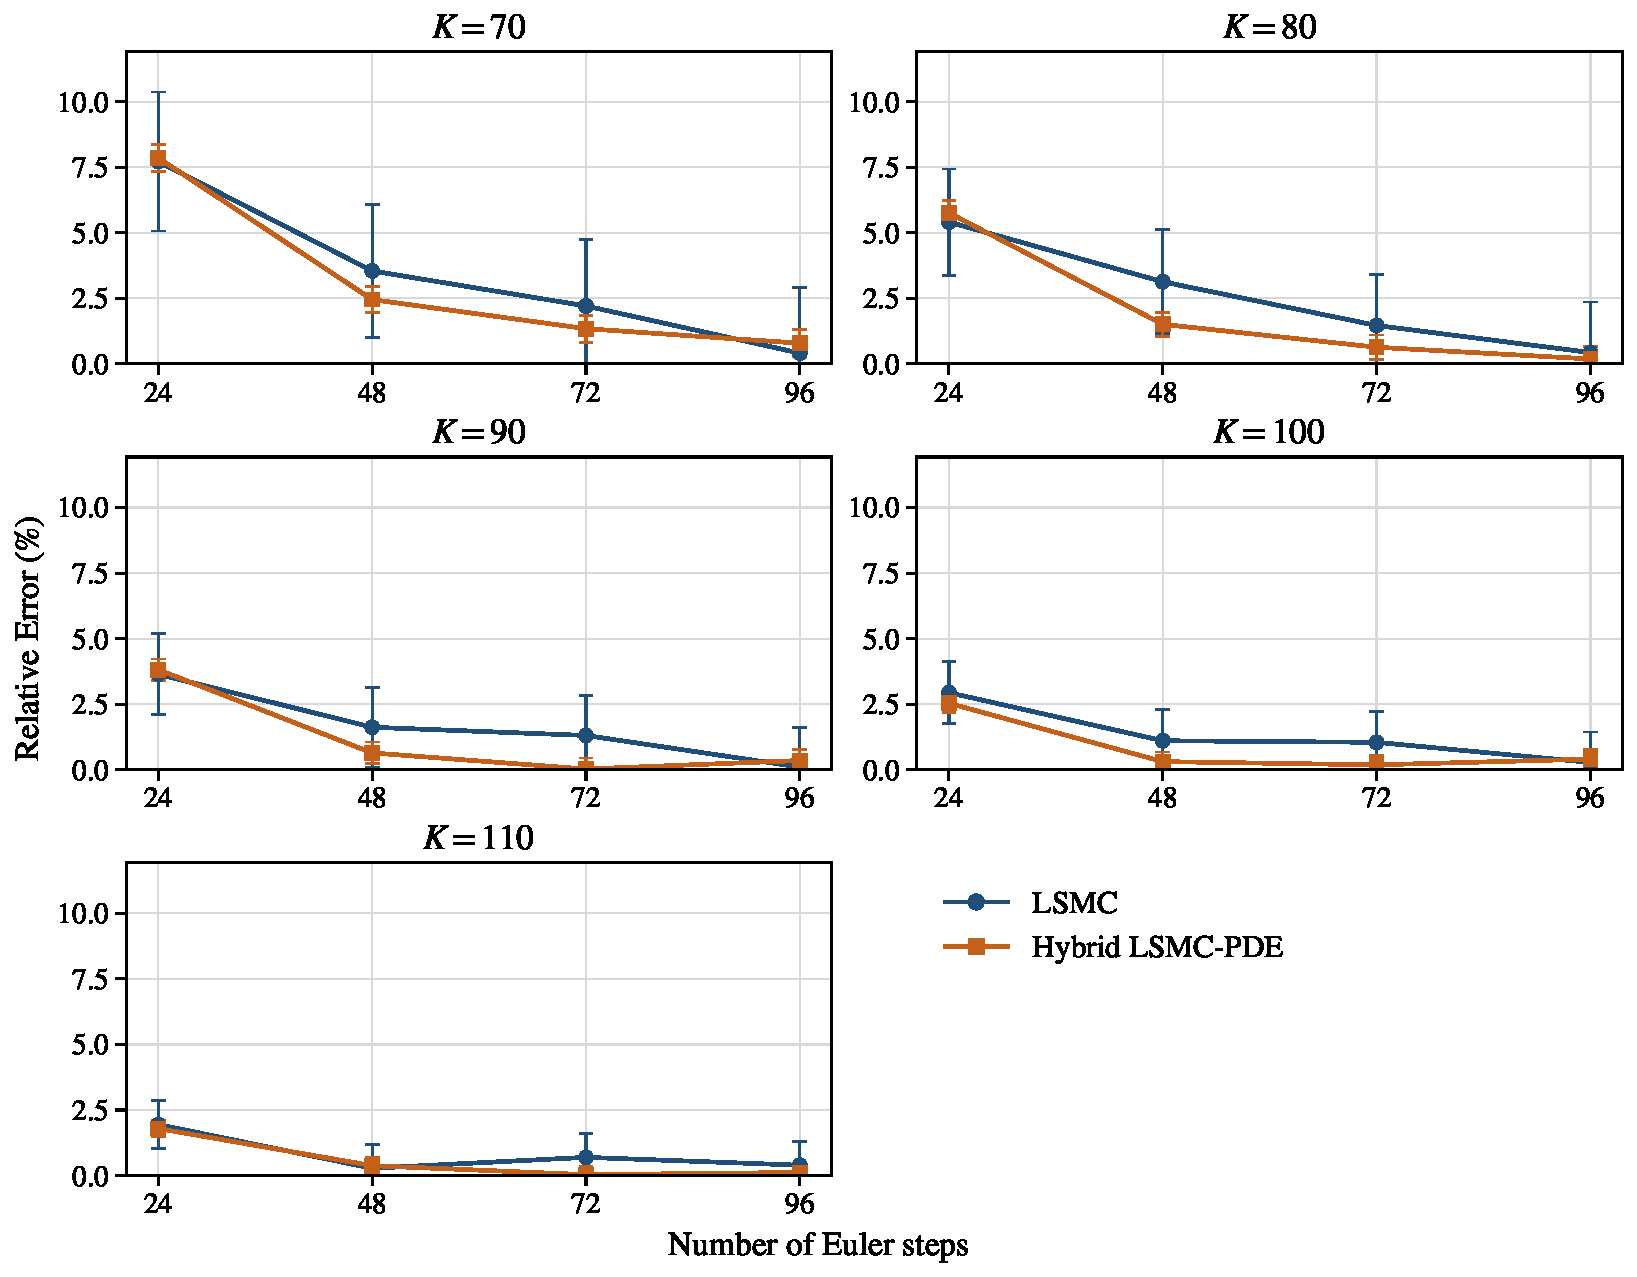
\includegraphics[width=\textwidth]{../Figures/step_sweep_60k_direct_relative_error.pdf}
\caption{Relative errors with associated error bars for $60{,}000$-path step-sweep experiment.}
\label{fig:step-sweep-60k}
\end{figure}

\FloatBarrier

\subsection{Fixed Euler step count and varying path budget}

The second experiment fixes the number of Euler time steps and varies the Monte Carlo
path budget. The reported path counts are $250,1000,5000,10000,20000,40000$,
and $60000$. Two discretization levels, $48$ and $60$ Euler steps, are
considered. This experiment focuses on sampling variation and regression error.

At $48$ Euler steps, the at-the-money strike $K=100$ gives relative errors of the plain LSMC estimator ranging from $1.105\%$ to $25.948\%$ over the path grid, while those of the Hybrid LSMC--PDE estimator range from $0.088\%$ to $11.118\%$. Figure~\ref{fig:path-sweep-48} shows the corresponding path-count sweep for all five strikes. 
%The corresponding pricing estimates are reported in Appendix~\ref{app:price-grids}.

\begin{figure}[H]
\centering
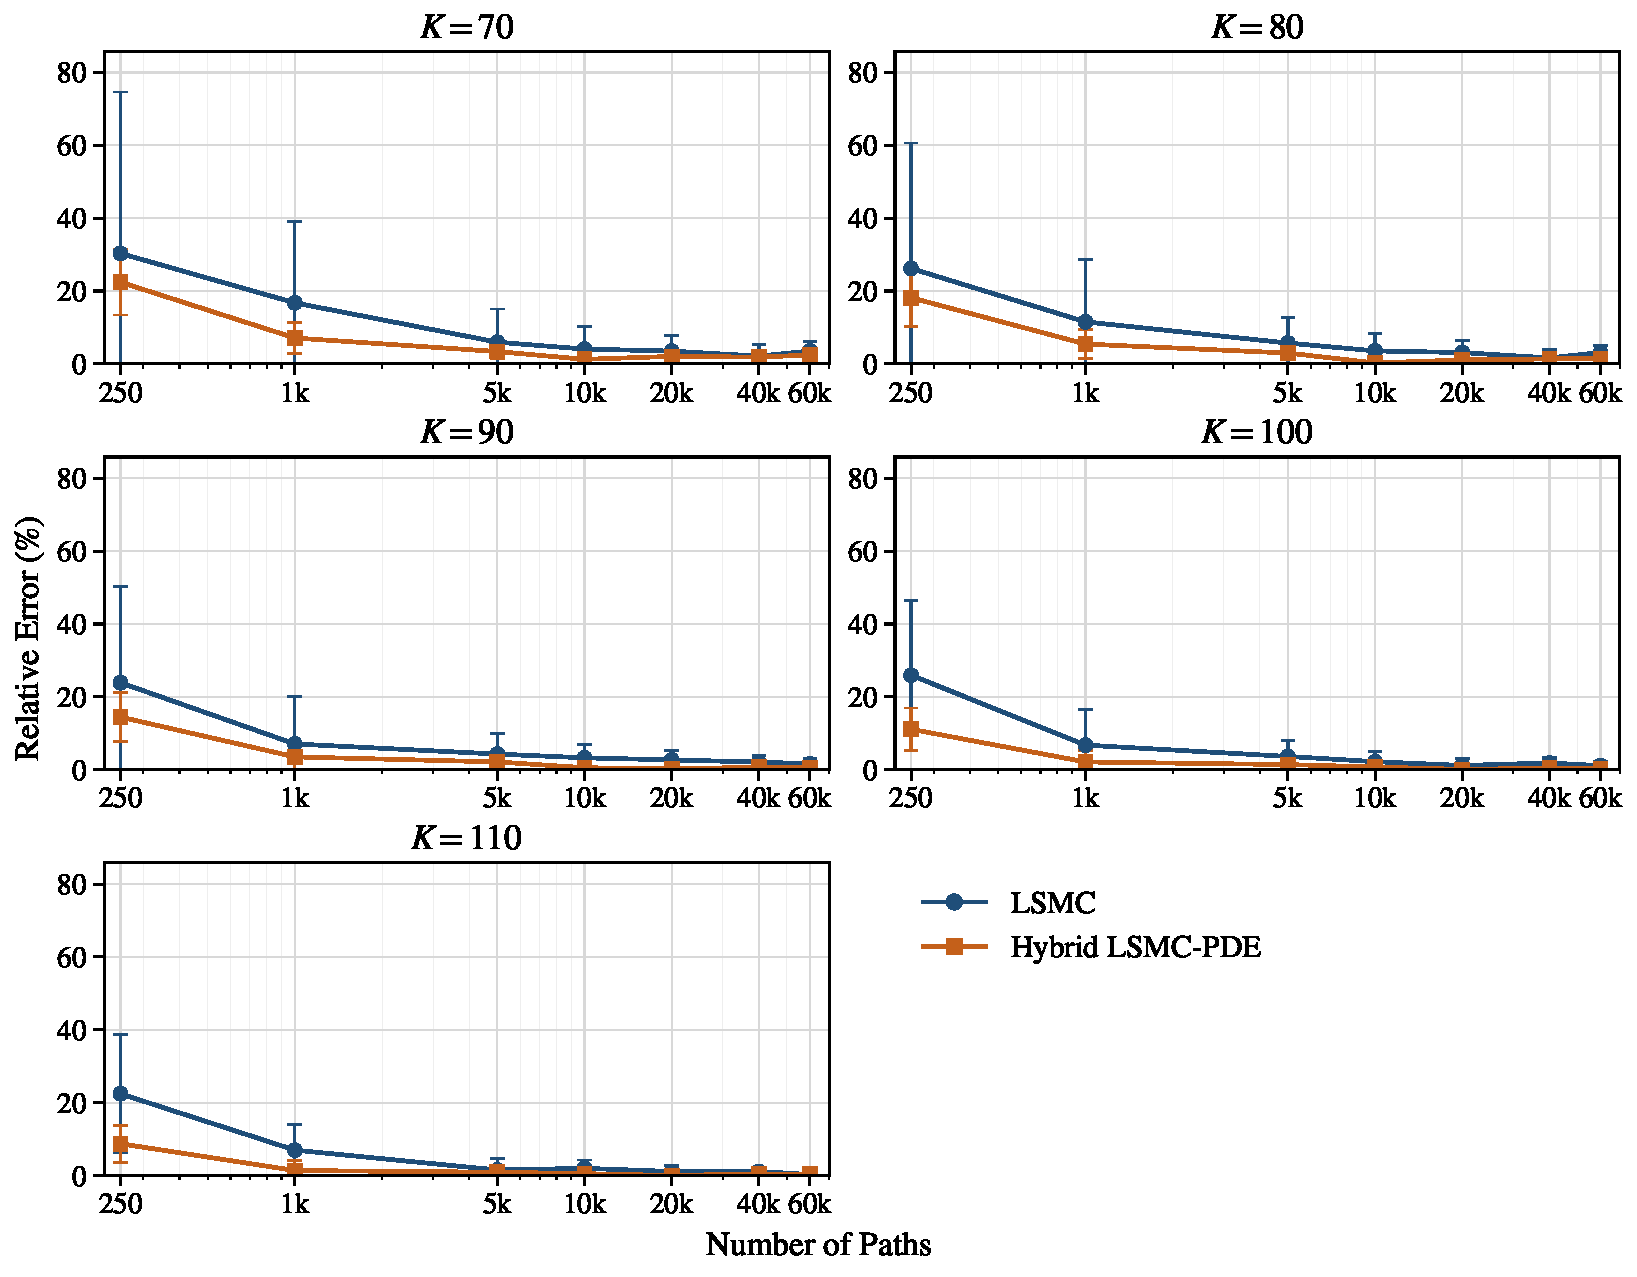
\includegraphics[width=\textwidth]{../Figures/path_sweep_steps48_direct_relative_error.pdf}
\caption{Relative errors with associated error bars for the fixed $48$-step path-sweep experiment.}
\label{fig:path-sweep-48}
\end{figure}

At $60$ Euler steps, the corresponding relative errors of the plain LSMC estimator range from $1.324\%$ to $28.932\%$, while those of the Hybrid LSMC--PDE estimator range from $0.049\%$ to $10.102\%$. Figure~\ref{fig:path-sweep-60} reports the corresponding path-count sweep for all five strikes. The reduction in relative error is most visible in the low- and moderate-path regimes, where the plain LSMC estimator is most affected by sampling noise.

\begin{figure}[H]
\centering
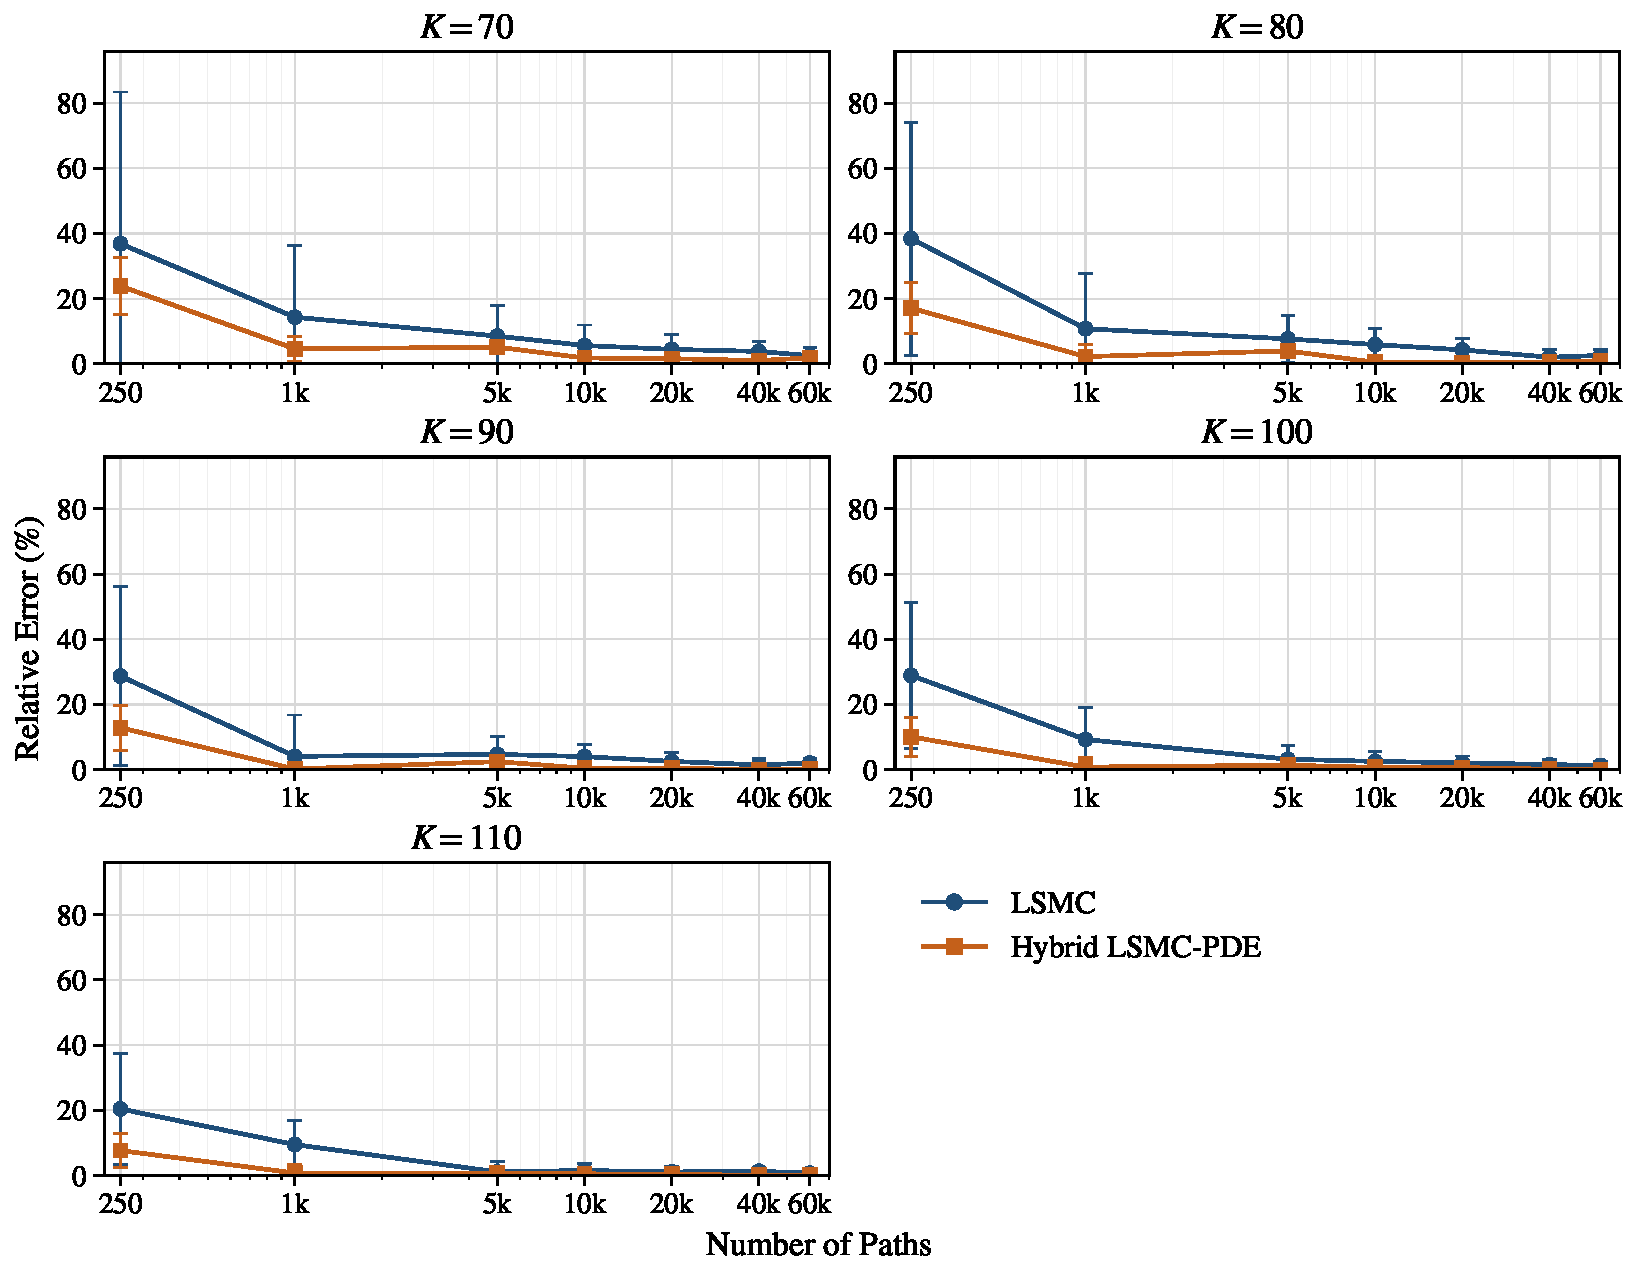
\includegraphics[width=\textwidth]{../Figures/path_sweep_steps60_direct_relative_error.pdf}
\caption{ Relative errors with associated error bars for the fixed $60$-step path-sweep experiment.}
\label{fig:path-sweep-60}
\end{figure}

\FloatBarrier

As shown in Figures~\ref{fig:step-sweep-20k}--\ref{fig:path-sweep-60}, the error bars are generally largest in the low-path experiments, especially for the plain LSMC estimator. In comparison, the Hybrid LSMC--PDE estimator is usually centered at lower relative errors and shows more stable error bars in the low and moderate path regimes. As the number of paths increases, the error bars shrink for both methods, and the difference between plain LSMC and Hybrid LSMC--PDE becomes smaller.

Overall, the experimental results are consistent with the conditional PDE step reducing the dimension of the continuation regression. Note that the comparisons are made against LSMC reference prices in Table~\ref{tab:reference-prices} obtained from large-scale simulations rather than exact prices. Since these benchmarks are naturally aligned with the LSMC methodology, the competitive performance of the Hybrid LSMC–PDE method is encouraging. One possible explanation is that, by exploiting model structure through a conditional PDE for the stock-price dependence rather than a full regression approximation of the continuation value, the Hybrid LSMC–PDE method may provide a more faithful representation of the exercise decision.


The complete set of estimated option prices is reported in Appendix~\ref{app:price-grids} and may serve as benchmark values for future studies. More specifically, the pricing estimates underlying Figures~\ref{fig:step-sweep-20k}--\ref{fig:path-sweep-60} are reported in Tables~\ref{tab:app-step-sweep-prices-20k}--\ref{tab:app-path-sweep-60-prices}, respectively.


\section{Conclusion}\label{sec:conclusion}

In this paper, we studied the pricing of Bermudan options under a GDMR model. Bermudan pricing requires the approximation of continuation values at each exercise date, and the two variance factors in the GDMR model make this regression problem more difficult than in a one-factor model. At the same time, the model has a useful one-way coupling; the variance factors can be simulated independently of the stock price. This structure leads naturally to the Hybrid LSMC--PDE method, since the stock-price direction can be handled conditionally while the remaining variance dependence is approximated by least-squares regression. We condition on the Brownian paths driving the variance factors and project the asset Brownian motion onto these drivers. Under this conditioning, each continuation step reduces to a one-dimensional problem in log-price. This gives the Gaussian conditional representation based on $Z_n$, $I_n$, $B_n$, and the variance values at the next exercise date, and leads to an FFT-based implementation of the conditional asset step. We also included that, for the CEV exponents $\delta_1,\delta_2 \in [1/2,1]$, the GDMR variance system has a unique strong solution and remains nonnegative. This property is needed since the construction of Hybrid LSMC--PDE relies on valid simulated variance paths.

We conducted the numerical study using a set of calibrated parameters from the literature. We compared plain LSMC with the Hybrid LSMC--PDE estimator across different Euler step counts and different numbers of Monte Carlo paths. Because no closed-form Bermudan benchmark is available for the GDMR model, the comparison was made against large-simulation plain LSMC reference prices. Within this setup, the Hybrid LSMC--PDE estimator produced smaller relative errors in many of the reported cases. The clearest gains appeared when the number of paths was low or moderate. The error bars also support this observation: they are generally
largest in the low-path experiments, especially for the plain LSMC estimator, while the
Hybrid LSMC--PDE estimator shows more stable error bars in the low and
moderate path regimes. 

These results suggest that the conditional PDE step may reduce the difficulty in approximating the continuation value in this model. For future work, we can test the method under additional calibrated parameter sets, consider alternative reference prices or bias-control procedures such as low-biased or dual estimators, and study other payoff types and early-exercise contracts.



\backmatter

\bmhead{Acknowledgements}
The authors thank Anatoliy Malyarenko for helpful discussions.

\section*{Declarations}

\subsection*{Funding}
Not applicable.

\subsection*{Conflict of interest/Competing interests}
The authors declare that they have no competing interests.

\subsection*{Ethics approval and consent to participate}
Not applicable.

\subsection*{Consent for publication}
Not applicable.

\subsection*{Data availability}
%The numerical data used to generate the tables and figures are included in the manuscript source %files.
No external datasets were used in this study. All numerical results were generated from simulated data based on the model specification described in the paper.
\subsection*{Materials availability}
Not applicable.

\subsection*{Code availability}
The computational code used for the numerical experiments in this study is available from the corresponding author upon reasonable request.

\subsection*{Author contributions}
MDK and YN contributed to the conceptualization, mathematical analysis, numerical design, interpretation of results, and manuscript preparation. All authors read and approved the final manuscript.
% Appendix price tables generated from canonical numerical CSV sources.
% Prices are rounded uniformly to three decimal places.
\begin{appendices}

\section{Proof of Theorem~\ref{thm:wellposed}}\label{app:proof-wellposed}

\noindent\textit{Proof.}
We first work with auxiliary equations on $\R$. For this purpose, the variance diffusion coefficients are extended by
$$
\sigma_i(x)=\xi_i(x^+)^{\delta_i},\qquad
x^+=\max\{x,0\},\qquad i=1,2.
$$
Once nonnegativity is proved, this extension is inactive because both variance factors stay in $[0,\infty)$. The auxiliary equations then coincide with the original system on the state space $\mathcal D$.

\emph{Step 1: construction of $v'$.}
Define
$$
b_2(x):=\kappa_2(\theta-x),\qquad
\sigma_2(x):=\xi_2(x^+)^{\delta_2},\qquad x\in\R.
$$
The drift $b_2$ is globally Lipschitz and has linear growth. The diffusion coefficient $\sigma_2$ is continuous, has at most linear growth, and satisfies the Yamada-Watanabe modulus condition by Assumption~\ref{ass:delta-range}. Therefore pathwise uniqueness holds for
$$
\dd v'_t=b_2(v'_t)\dd t+\sigma_2(v'_t)\dd W^{(3)}_t,
\qquad v'_0\ge0;
$$
see \cite{yamada1971uniqueness} and \cite[Ch.~5]{karatzas1991brownian}. Since the coefficients are continuous with linear growth, weak existence holds. Weak existence together with pathwise uniqueness yields a unique strong solution by the Yamada-Watanabe theorem.

It remains to show that the solution does not leave the nonnegative half-line. At the boundary,
$$
\sigma_2(0)=0,\qquad b_2(0)=\kappa_2\theta\ge0.
$$
Moreover, on the negative extension one has
$$
\sigma_2(x)=0,\qquad b_2(x)=\kappa_2(\theta-x)\ge0,\qquad x\le0.
$$
Thus the diffusion has no outward noise at the boundary and the drift points inward on the negative side. The standard one-dimensional stochastic invariance criterion for closed intervals therefore yields
$$
v'_t\ge0,\qquad 0\le t\le T,\quad \Q\text{-a.s.}
$$

\emph{Step 2: construction of $v$.}
Having constructed $v'$, define
$$
b_1(t,x):=\kappa_1(v'_t-x),\qquad
\sigma_1(x):=\xi_1(x^+)^{\delta_1}.
$$
For $m\ge1$, set
$$
\tau_m:=\inf\{t\ge0:v'_t>m\}\wedge T.
$$
Since $v'$ has continuous paths on $[0,T]$, we have $\tau_m\uparrow T$
almost surely. On $[0,\tau_m]$, the drift $b_1$ is progressively
measurable, Lipschitz in $x$ with constant $\kappa_1$, and satisfies
$$
|b_1(t,x)|\le\kappa_1(m+|x|).
$$
The diffusion coefficient $\sigma_1$ is continuous, has at most linear growth,
and satisfies the Yamada-Watanabe modulus condition. The localized
one-dimensional existence and pathwise-uniqueness theorem for SDEs with
progressive random coefficients, obtained by the same Yamada-Watanabe argument
after localization, therefore gives a unique strong stopped solution of
$$
\dd v_t=b_1(t,v_t)\dd t+\sigma_1(v_t)\dd W^{(2)}_t,
\qquad t\le\tau_m.
$$
The possible correlation between $W^{(2)}$ and $W^{(3)}$ is immaterial here:
pathwise uniqueness compares solutions driven by the same Brownian vector and
the same realized input path $v'$. By pathwise uniqueness, the stopped
solutions are compatible on overlaps. Letting $m\to\infty$ gives a unique
strong solution for $v$ on $[0,T]$.

The same invariance argument gives nonnegativity. Since $v'_t\ge0$,
$$
b_1(t,0)=\kappa_1v'_t\ge0,\qquad \sigma_1(0)=0.
$$
On the negative extension,
$$
b_1(t,x)=\kappa_1(v'_t-x)\ge0,\qquad
\sigma_1(x)=0,\qquad x\le0.
$$
Hence the closed half-line is invariant and
$$
v_t\ge0,\qquad 0\le t\le T,\quad \Q\text{-a.s.}
$$

\emph{Step 3: construction of $S$.}
The process $v$ is continuous and finite on the compact interval $[0,T]$.
Therefore
$$
\int_0^T v_s\,\dd s<\infty\qquad \Q\text{-a.s.}
$$
The asset equation is linear in $S$, and its unique strong solution is
$$
S_t
=S_0
\exp\!\left(
\int_0^t \Bigl(r-\tfrac12 v_s\Bigr)\dd s
+\int_0^t \sqrt{v_s}\,\dd W_s^{(1)}
\right).
$$
Thus $S_t>0$ for all $t\in[0,T]$ whenever $S_0>0$.

The auxiliary positive-part extension is inactive along the constructed variance
paths, because $v_t,v'_t\ge0$. Hence the constructed solution solves the
original nonnegative-state system \eqref{eq:gdmr}. Pathwise uniqueness for the
auxiliary triangular system gives pathwise uniqueness for \eqref{eq:gdmr}.

Finally, existence and pathwise uniqueness for every deterministic initial state
imply uniqueness in law. Since the coefficients are time homogeneous, the
standard strong Markov property for well-posed time-homogeneous SDEs gives that
the solution is a time-homogeneous strong Markov process on $\mathcal D$.
\hfill$\square$

\section{Pricing estimates for the numerical experiments}\label{app:price-grids}
This appendix reports the Bermudan put pricing estimates corresponding to the numerical experiments in Section~\ref{sec:numerical}. The pricing estimates reported in Tables~\ref{tab:app-step-sweep-prices-20k}--\ref{tab:app-path-sweep-60-prices} correspond to the numerical experiments in Figures~\ref{fig:step-sweep-20k}--\ref{fig:path-sweep-60}. The associated large-simulation LSMC reference prices are reported in Table~\ref{tab:reference-prices}. All entries in Tables~\ref{tab:app-step-sweep-prices-20k}--\ref{tab:app-path-sweep-60-prices} are rounded to three decimal places. The label LSMC denotes the plain least-squares Monte Carlo estimator, and Hybrid denotes the Hybrid LSMC--PDE estimator. 



\begin{table}[htbp]
\centering
\caption{Pricing estimates in the fixed-path step-sweep experiment with $20{,}000$ paths. Prices are rounded to three decimal places.}
\label{tab:app-step-sweep-prices-20k}
\footnotesize
\setlength{\tabcolsep}{3pt}
\begin{tabular}{lrrrr}
\toprule
Method/step & 24 & 48 & 72 & 96 \\
\midrule
LSMC $K=70$ & 2.741 & 2.612 & 2.579 & 2.536 \\
Hybrid $K=70$ & 2.711 & 2.575 & 2.547 & 2.565 \\
LSMC $K=80$ & 4.634 & 4.433 & 4.409 & 4.396 \\
Hybrid $K=80$ & 4.528 & 4.345 & 4.307 & 4.339 \\
LSMC $K=90$ & 7.341 & 7.129 & 7.068 & 7.080 \\
Hybrid $K=90$ & 7.172 & 6.957 & 6.905 & 6.956 \\
LSMC $K=100$ & 11.138 & 10.807 & 10.816 & 10.837 \\
Hybrid $K=100$ & 10.898 & 10.673 & 10.607 & 10.679 \\
LSMC $K=110$ & 16.241 & 15.920 & 15.894 & 15.798 \\
Hybrid $K=110$ & 15.953 & 15.747 & 15.676 & 15.768 \\
\botrule
\end{tabular}
\end{table}

\begin{table}[htbp]
\centering
\caption{Pricing estimates in the fixed-path step-sweep experiment with $60{,}000$ paths. Prices are rounded to three decimal places.}
\label{tab:app-step-sweep-prices-60k}
\footnotesize
\setlength{\tabcolsep}{3pt}
\begin{tabular}{lrrrr}
\toprule
Method/step & 24 & 48 & 72 & 96 \\
\midrule
LSMC $K=70$ & 2.718 & 2.612 & 2.579 & 2.533 \\
Hybrid $K=70$ & 2.721 & 2.585 & 2.557 & 2.543 \\
LSMC $K=80$ & 4.531 & 4.434 & 4.362 & 4.318 \\
Hybrid $K=80$ & 4.547 & 4.364 & 4.326 & 4.307 \\
LSMC $K=90$ & 7.195 & 7.055 & 7.033 & 6.949 \\
Hybrid $K=90$ & 7.207 & 6.987 & 6.940 & 6.918 \\
LSMC $K=100$ & 10.996 & 10.800 & 10.794 & 10.712 \\
Hybrid $K=100$ & 10.953 & 10.715 & 10.662 & 10.639 \\
LSMC $K=110$ & 16.050 & 15.788 & 15.853 & 15.806 \\
Hybrid $K=110$ & 16.026 & 15.803 & 15.749 & 15.725 \\
\botrule
\end{tabular}
\end{table}

\begin{table}[htbp]
\centering
\caption{Pricing estimates in the fixed 48-step path-sweep experiment. Prices are rounded to three decimal places.}
\label{tab:app-path-sweep-48-prices}
\footnotesize
\setlength{\tabcolsep}{2.5pt}
\begin{tabular}{lrrrrrrr}
\toprule
Method/path count & 250 & 1,000 & 5,000 & 10,000 & 20,000 & 40,000 & 60,000 \\
\midrule
LSMC $K=70$ & 3.288 & 2.946 & 2.673 & 2.625 & 2.612 & 2.576 & 2.612 \\
Hybrid $K=70$ & 3.089 & 2.702 & 2.608 & 2.554 & 2.575 & 2.570 & 2.585 \\
LSMC $K=80$ & 5.425 & 4.795 & 4.545 & 4.452 & 4.433 & 4.369 & 4.434 \\
Hybrid $K=80$ & 5.079 & 4.533 & 4.427 & 4.310 & 4.345 & 4.357 & 4.364 \\
LSMC $K=90$ & 8.601 & 7.433 & 7.241 & 7.169 & 7.129 & 7.088 & 7.055 \\
Hybrid $K=90$ & 7.946 & 7.187 & 7.090 & 6.903 & 6.957 & 6.992 & 6.987 \\
LSMC $K=100$ & 13.454 & 11.404 & 11.072 & 10.918 & 10.807 & 10.881 & 10.800 \\
Hybrid $K=100$ & 11.870 & 10.910 & 10.833 & 10.601 & 10.673 & 10.730 & 10.715 \\
LSMC $K=110$ & 19.278 & 16.843 & 15.985 & 16.057 & 15.920 & 15.921 & 15.788 \\
Hybrid $K=110$ & 17.120 & 15.962 & 15.889 & 15.660 & 15.747 & 15.819 & 15.803 \\
\botrule
\end{tabular}
\end{table}

\begin{table}[htbp]
\centering
\caption{Pricing estimates in the fixed 60-step path-sweep experiment. Prices are rounded to three decimal places.}
\label{tab:app-path-sweep-60-prices}
\footnotesize
\setlength{\tabcolsep}{2.5pt}
\begin{tabular}{lrrrrrrr}
\toprule
Method/path count & 250 & 1,000 & 5,000 & 10,000 & 20,000 & 40,000 & 60,000 \\
\midrule
LSMC $K=70$ & 3.452 & 2.884 & 2.738 & 2.665 & 2.635 & 2.619 & 2.587 \\
Hybrid $K=70$ & 3.125 & 2.639 & 2.653 & 2.568 & 2.563 & 2.549 & 2.570 \\
LSMC $K=80$ & 5.950 & 4.762 & 4.629 & 4.553 & 4.484 & 4.387 & 4.411 \\
Hybrid $K=80$ & 5.034 & 4.396 & 4.470 & 4.321 & 4.318 & 4.321 & 4.342 \\
LSMC $K=90$ & 8.936 & 7.227 & 7.270 & 7.222 & 7.120 & 7.045 & 7.084 \\
Hybrid $K=90$ & 7.836 & 6.957 & 7.115 & 6.910 & 6.910 & 6.939 & 6.957 \\
LSMC $K=100$ & 13.773 & 11.673 & 11.026 & 10.955 & 10.910 & 10.850 & 10.823 \\
Hybrid $K=100$ & 11.761 & 10.596 & 10.831 & 10.604 & 10.610 & 10.666 & 10.677 \\
LSMC $K=110$ & 18.962 & 17.240 & 15.920 & 15.991 & 15.918 & 15.952 & 15.860 \\
Hybrid $K=110$ & 16.953 & 15.621 & 15.863 & 15.659 & 15.680 & 15.755 & 15.757 \\
\botrule
\end{tabular}
\end{table}

\end{appendices}

\bibliography{references}

\end{document}
